\subsection{IFIT2 Localisation in the Context of RSV IBs} \label{subsec:IFIT2 Localisation in the Context of RSV IBs}
\subsubsection{Human Infection}
%i2a a549 hrsv
Cell Line: A549 \newline
Treatment: hRSV \newline
Detecting magenta: endogenous human IFIT2  \newline
Detecting cyan: human IB \newline

Nascent human IFIT2 shows 3 phenotypes with regards to colocalization with human RSV N. It seems to colocalise to the edge of the IB structure, with a partial signal also being detected in the inner edge of the structure (top panel); it completely colocalises to the N staining (middle panel; could be because the section is going through the top of the IB sphere); or forms inclusion inside the IB structure (bottom panel. 

\begin{figure}
    \centering
    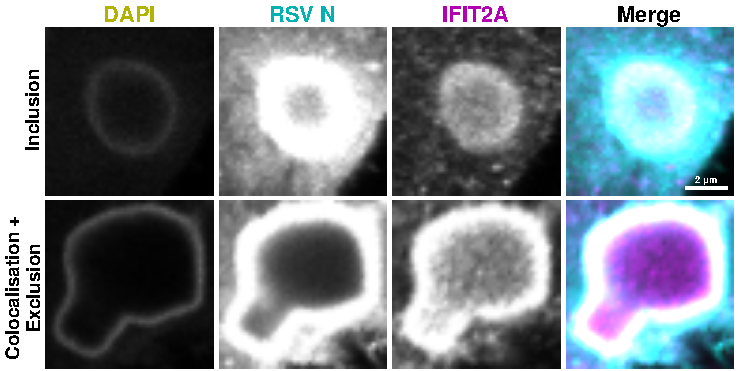
\includegraphics[width=1\linewidth]{10. Chapter 5/Figs/01. Infection/01. i2a a549 hrsv n.pdf}
    \caption[i2a a549 hrsv n]{i2a a549 hrsv n}
    \label{fig:i2a a549 hrsv n}
\end{figure}

Cell Line: A549 \newline
Treatment: hRSV \newline
Detecting magenta: endogenous human IFIT2  \newline
Detecting cyan: human IB \newline

Nascent human IFIT2 colocalises with the ring structure (outlined by RSV P staining) and to the inner edge of the IB.

\begin{figure}
    \centering
    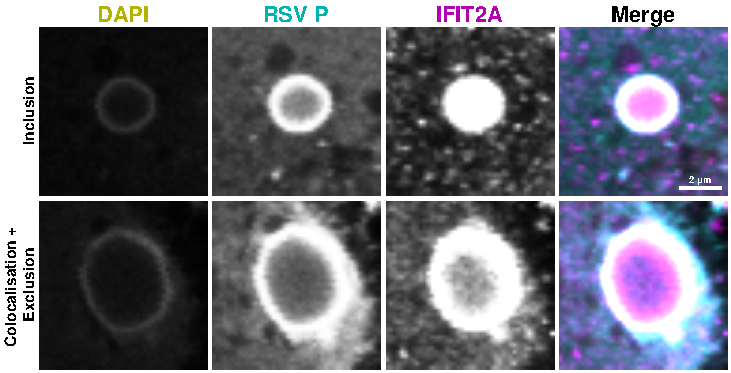
\includegraphics[width=1\linewidth]{10. Chapter 5/Figs/01. Infection/02. i2a a549 hrsv p.pdf}
    \caption[i2a a549 hrsv p]{i2a a549 hrsv p}
    \label{fig:i2a a549 hrsv p}
\end{figure}

Cell Line: A549 \newline
Treatment: hRSV \newline
Detecting magenta: endogenous human IFIT2  \newline
Detecting cyan: human IB \newline

With regards of colocalization with human RSV M2/1 protein, human IFIT2 seems to either form inclusion, which has a signal decrease towards the middle of the IB structure (top panel), or seems to strongly colocalise with the ring structure highlighted by M2/1 staining (bottom 2 panels; there also seems to be IFIT2 signal concentration on the inner edge of the IB structure).

\begin{figure}
    \centering
    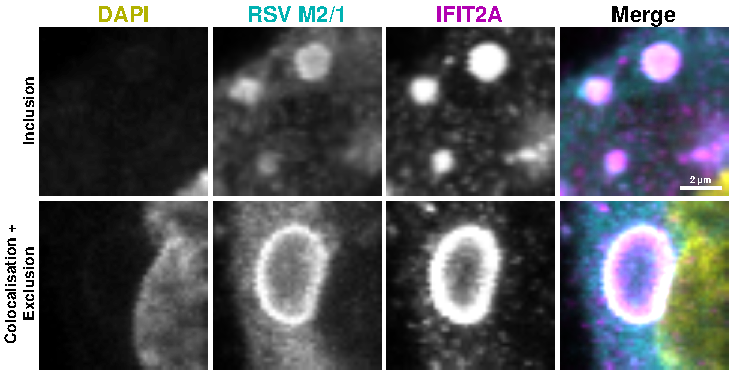
\includegraphics[width=1\linewidth]{10. Chapter 5/Figs/01. Infection/03. i2a a549 hrsv m21.pdf}
    \caption[i2a a549 hrsv m21]{i2a a549 hrsv m21}
    \label{fig:i2a a549 hrsv m21}
\end{figure}

%i2a beas2b hrsv
Cell Line: BEAS2B \newline
Treatment: hRSV \newline
Detecting magenta: endogenous human IFIT2  \newline
Detecting cyan: human IB \newline

\begin{figure}
    \centering
    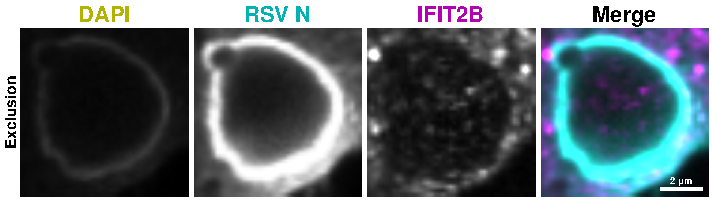
\includegraphics[width=1\linewidth]{10. Chapter 5/Figs/01. Infection/04. i2b a549 hrsv n.pdf}
    \caption[i2a beas2b hrsv]{i2a beas2b hrsv}
    \label{fig:i2a beas2b hrsv}
\end{figure}

%i2b a549 hrsv
Cell Line: A549 \newline
Treatment: hRSV \newline
Detecting magenta: endogenous human IFIT2  \newline
Detecting cyan: human IB \newline

Endogenous human IFIT2 is either partially excluded (top panel; decrease of intra IB signal compared to cytoplasmic signal) or completely excluded (bottom panel) from the human IB structure.

\begin{figure}
    \centering
    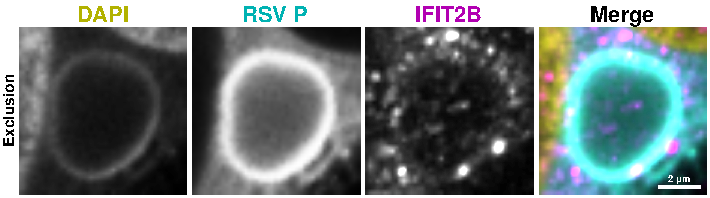
\includegraphics[width=1\linewidth]{10. Chapter 5/Figs/01. Infection/05. i2b a549 hrsv p.pdf}
    \caption[i2b a549 hrsv n]{i2b a549 hrsv n}
    \label{fig:i2b a549 hrsv n}
\end{figure}

Cell Line: A549 \newline
Treatment: hRSV \newline
Detecting magenta: endogenous human IFIT2  \newline
Detecting cyan: human IB  \newline

We observe similar pattern of staining to what was observed with N stained human IBs. IFIT2 signal is either partially or totally excluded from the IB structure.

\begin{figure}
    \centering
    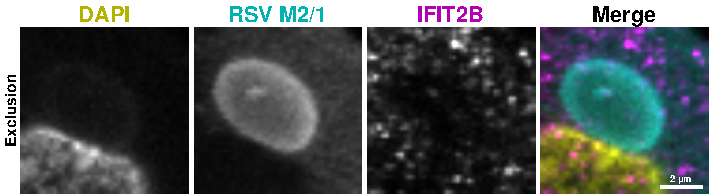
\includegraphics[width=1\linewidth]{10. Chapter 5/Figs/01. Infection/06. i2b a549 hrsv m21.pdf}
    \caption[i2b a549 hrsv m21]{i2b a549 hrsv m21}
    \label{fig:i2b a549 hrsv m21}
\end{figure}

Cell Line: A549 \newline
Treatment: hRSV \newline
Detecting magenta: endogenous human IFIT2  \newline
Detecting cyan: human IB \newline

Endogenous human IFIT2 seems to be excluded from hRSV IBs.

\begin{figure}
    \centering
    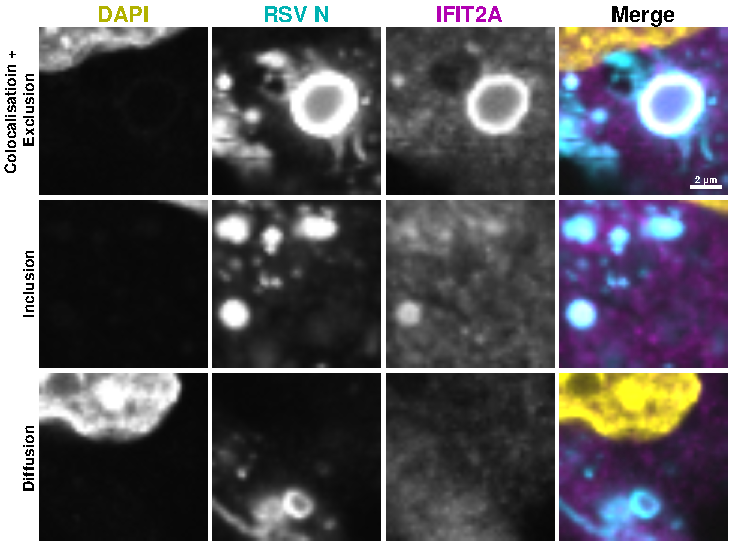
\includegraphics[width=1\linewidth]{10. Chapter 5/Figs/01. Infection/07. i2a beas2b.pdf}
    \caption[i2a beas2b]{i2a beas2b}
    \label{fig:i2a beas2b}
\end{figure}

\subsubsection{Bovine Infection}
%i2a mdbk brsv
Cell Line: MDBK \newline
Treatment: bRSV + bIFNa \newline
Detecting magenta: endogenous bovine IFIT2  \newline
Detecting cyan: bovine IB \newline

Nascent bovine IFIT2 colocalization with regards of N stained bRSV IBs seems to strongly associate with the ring of the structure.

\begin{figure}
    \centering
    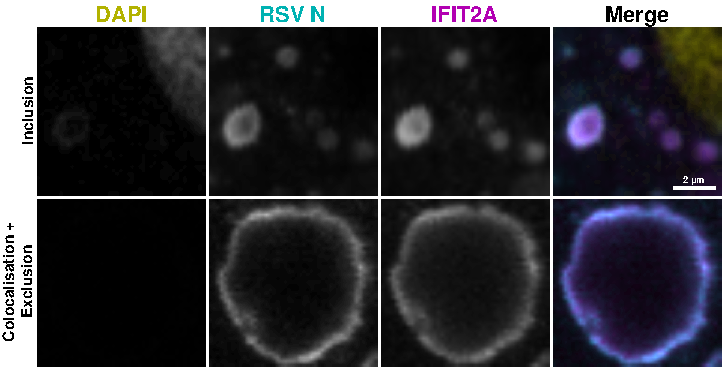
\includegraphics[width=1\linewidth]{10. Chapter 5/Figs/01. Infection/08. i2a mdbk brsv.pdf}
    \caption[i2a mdbk brsv]{i2a mdbk brsv}
    \label{fig:i2a mdbk brsv}
\end{figure}

%i2b mdbk brsv
Cell Line: MDBK \newline
Treatment: bRSV + bIFNa \newline
Detecting magenta: endogenous bovine IFIT2  \newline
Detecting cyan: bovine IB \newline

Endogenous bovine IFIT2 localisation with respect to the bovine inclusion bodies shows a few different phenotypes. We see partial exclusion (to panel; signal still present in the middle of the IB structure), exclusion from IB ring and the inner IB edge (middle panel; highlighted with arrow) with IBAG-like concentrations inside the structure; and diffusion through the IB structure (bottom panel). These phenotypes are similar to what is observed during RSV infection of human but especially bovine IFIT3 and IFIT5.

\begin{figure}
    \centering
    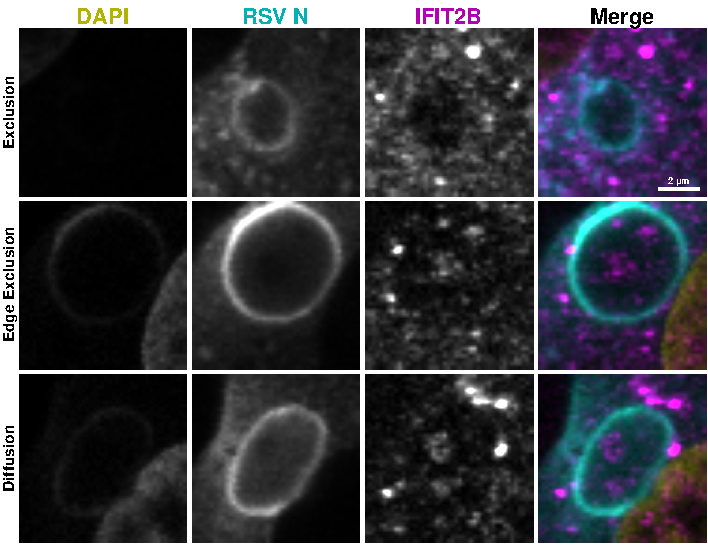
\includegraphics[width=1\linewidth]{10. Chapter 5/Figs/01. Infection/09. i2b mdbk brsv.pdf}
    \caption[i2b mdbk brsv]{i2b mdbk brsv}
    \label{fig:i2b mdbk brsv}
\end{figure}

\subsubsection{Summary} \label{Summary-i2-infection}
Nascent human IFIT2 during hRSV infection consistently localises to the IB structure. It seems to have preference for the ring and the inner edge of the structure; however, we have seen it as homogenous inclusion as well. Endogenous bovine IFIT2 colocalises to the ring of the IB during bRSV infection.

Nascent human IFIT2 shows full or partial exclusion from human IBs during human RSV infection. Nascent bovine IFIT2 during bRSV infections shows 3 different phenotypes. We observed partial exclusion; exclusion from the IB ring and inner edge with IBAG-like inclusions; and diffusion through the IB structure. This staining is similar to what is observed with bovine IFIT3 and IFIT5 during bRSV infection.